\documentclass[10pt,a4paper]{beamer}

\usetheme{Berkeley}
\usecolortheme{sidebartab}

\usepackage{graphicx}
\usepackage{movie15,media9}
\setbeamertemplate{caption}[numbered]

\begin{document}
	\setbeamertemplate{sidebar left}{}
	\title{Progress Presentation-I}
	\subtitle{e-Yantra Summer Internship-2018 \\ $ $\textbf{A System for Solving Jigsaw Puzzle using Multiple Robots}$ $}
	\author{$ $Aniket Anantraj Navlur$ $\\$ $Ashis kumar Maharana$ $\\$ $Kiran S Patil$ $\\ \vspace{1em}
	Mentors: \\$ $Abhinav Sarkar, Kalind Karia$ $}
	\institute{IIT Bombay}
	\date{\today}
	%\addtobeamertemplate{sidebar left}{}{\includegraphics[scale = 0.3]{logowithtext.png}}
	\frame{\titlepage}

\setbeamertemplate{sidebar left}[sidebar theme]
\section{Overview of Project}
\begin{frame}{Overview of Project}
	
	\begin{itemize}
		\item Project Name: A System for Solving Jigsaw Puzzle using Multiple Robots
		\item Objective:
		\begin{itemize}
			\item To develop an autonomous system that can solve any Jigsaw Puzzle given its image using multiple robots 
		\end{itemize}
		\item Deliverables:
		\begin{enumerate}
			\item Go-to-Goal controller for robot in a given frame
			\item Autonomous solving of any Jigsaw Puzzle given just its image
			\item Proper documentation and report on the system
		\end{enumerate}
	\end{itemize}
\end{frame}

\section{Overview of Task}
\begin{frame}{Overview of Task}
	\begin{tabular}{| c | p{17.5 em} | c |}\hline
		\textbf{Task No.} & \hspace{7em}\textbf{Task} & \textbf{Deadline} \\
		& & (in Days)\\\hline
		1 &\small{ Python, OpenCV, Firebird V Intro,\hspace{5 em}Xbee Communication} & 3 \\\hline
		2 &\small{ Pose and orientation calculation of 2 Firebird robots using color/Aruco markers }& 4\\\hline
		3 &\small{ Programming the Go-To-Goal Controller for single Firebird V robot. Tuning the PID\hspace{3 em} values to perfection }& 4\\\hline
		4 &\small{ Implementing path planning with Firebird V where obstacles have been placed in arena }& 3\\\hline
		5 &\small{ Detection of jigsaw puzzle blocks using\hspace{3 em}Template Matching} & 2\\\hline
		6 &\small{ Pick and place of blocks - gripper mechanism building }& 4\\\hline
		7 &\small{ Implementing the entire solution for a given\hspace{3 em}jigsaw puzzle }& 5\\\hline
		8 &\small{ Documentation and reporting results }& 4\\\hline
	\end{tabular}
\end{frame}

\section{Task Accomplished}
\begin{frame}{Task Accomplished}
\begin{itemize}
\item Established communication with the robot using XBee\pause
\item Found the pose and orientation of the robot using ArUco markers
\begin{figure}
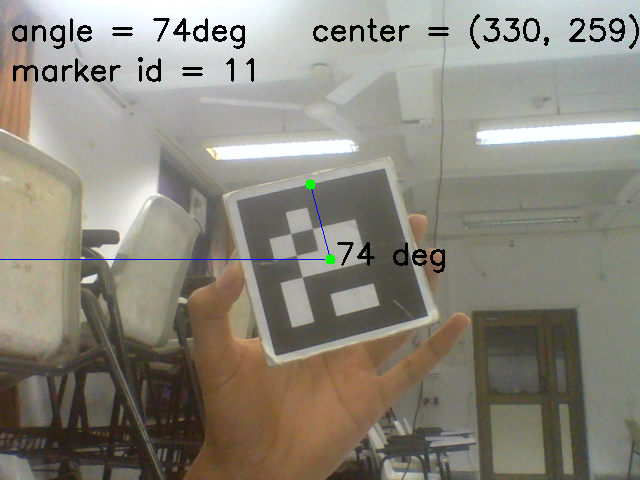
\includegraphics[height=0.6\textheight, width=0.7\textwidth]{image_screenshot2.png}\caption{ArUco id, center position, orientation}
\end{figure}
\end{itemize}
\end{frame}
\begin{frame}{Task Accomplished}
\begin{itemize}
\item Formed the data packets to be sent, received and parsed correctly\pause
\begin{figure}
\includegraphics[height=0.45\textheight, width=0.65\textwidth]{capture.png}\caption{Data Packets}
\end{figure}
\small{The data packet is formed by the following values}
\small{$<T|tar_x|tar_y|P|kp|ki|kd|R|head_x|head_y|tail_x|tail_y|A|deg|>$}\pause
\item Tuned the PID values to perfection\pause
\item Developed a Go-To-Goal controller for multiple robots
\end{itemize}
\end{frame}

\section{Videos}
\begin{frame}{Videos}
\begin{columns}
\column{0.5\textwidth}
\begin{figure}

\includemedia[
     width=5cm,height=3cm,
     activate=pageopen,
     addresource=image.mp4,
     flashvars={
         source=image.mp4
        &autoPlay=false
     }
]{}{VPlayer.swf}\vspace{-1 em}\caption{\small{PID tuned}}
\end{figure}\vspace{-2 em}
\begin{figure}
\includemedia[
     width=5cm,height=3cm,
     activate=pageopen,
     addresource=imgi.mp4,
     flashvars={
         source=imgi.mp4
        &autoPlay=false
     }
]{}{VPlayer.swf}\vspace{-1 em}\caption{\small{showing error angle being corrected}}
\end{figure}
\column{0.5\textwidth}
\begin{figure}

\includemedia[
     width=5cm,height=5cm,
     activate=pageopen,
     addresource=img.mp4,
     flashvars={
         source=img.mp4
        &autoPlay=false
     }
]{}{VPlayer.swf}\caption{travelling to the nearest node}
\end{figure}

\end{columns}

\end{frame}

\section{Challenges Faced}
\begin{frame}{Challenges Faced}
	\begin{itemize}
		\item Determining the angle of ArUco Marker in the frame with proper resolution\pause
		\item Finding the right library for serial communication\pause
		\item Understanding the parameters of Xbee('DH','DL','MY',channel$=$'C', API, AT, etc...)\pause
		\item Creating data packets to hold the information about robot (its orientation, position, etc...) and parsing it once received by the robot.
	\end{itemize}
\end{frame}

\section{Future Plans}
\begin{frame}{Future Plans}
	\begin{itemize}
		\item Path Planning of Robot\pause
		\item Designing and building Gripper Mechanism to pick and place Jigsaw blocks and implementing the entire solution for Jigsaw puzzle\pause
		\item Solve a Multi-Robot Cooperative Box-pushing problem
	\end{itemize}
\end{frame}


\section{Thank You}
\begin{frame}{Thank You}
	\centering THANK YOU !!!
\end{frame}
\end{document}
